En esta sección se detallarán los casos de uso y escenarios pertenecientes al subsistema de gestión de usuarios.
La figura \ref{fig:casos_uso_subsistema_usuarios} muestra el diagrama de casos de dicho subsistema.

\begin{figure}[h]
\centering
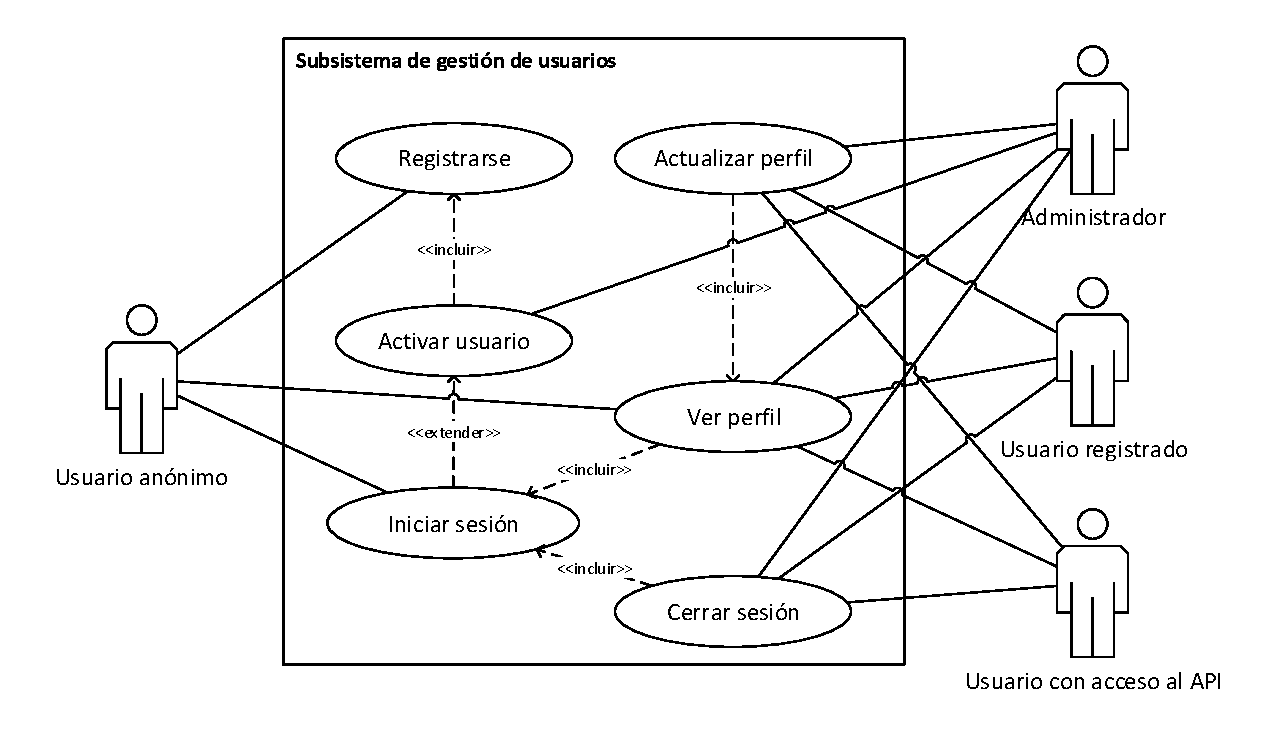
\includegraphics[width=\textwidth]{casos_uso/diagrama_casos_uso_usuarios}
\caption{Diagrama de casos de uso del subsistema de gestión de usuarios}
\label{fig:casos_uso_subsistema_usuarios}
\end{figure}


\subsubsection{Caso de uso ``registrarse''}
\begin{description}
\item[Descripción] 				El usuario no dispone de una cuenta en el sistema y quiere crear una.
\item[Actores]					Cualquier usuario anónimo.
\item[Escenario principal]	 	\hfill
								\begin{enumerate}
								\item El usuario accede al formulario de registro.
								\item Una vez en el formulario de registro, el usuario rellena todos los campos requeridos.
								\item Si el usuario lo decide también puede rellenar los campos opcionales.
								\item Tras rellenar los campos el usuario pulsa el botón de registro.
								\item El sistema guarda los datos y crea la nueva cuenta de usuario con estado bloqueado.
								\end{enumerate}
\item[Escenario alternativo 1]	El usuario no rellena todos los campos necesarios.
								\begin{enumerate}
								\item Cuando el usuario pulse el botón para completar el registro el sistema notificará del error.
								\item Se continuará desde el punto 2 del escenario principal.
								\end{enumerate}
\item[Escenario alternativo 2]	El nombre de usuario ya existe en el sistema.
								\begin{enumerate}
								\item Cuando el usuario pulse el botón para completar el registro el sistema notificará del error.
								\item Se continuará desde el punto 2 del escenario principal.
								\end{enumerate}
\item[Escenario alternativo 3]	El email de usuario ya existe en el sistema.
								\begin{enumerate}
								\item Cuando el usuario pulse el botón para completar el registro el sistema notificará del error.
								\item Se continuará desde el punto 2 del escenario principal.
								\end{enumerate}
\end{description}


\subsubsection{Caso de uso ``activar usuario''}
\begin{description}
\item[Descripción] 				El administrador activa una cuenta de un usuario para que éste pueda utilizarla.
\item[Actores]					El administrador del sistema.
\item[Precondiciones]			La cuenta de usuario debe ser registrada previamente en el sistema.
\item[Escenario principal]	 	\hfill
								\begin{enumerate}
								\item El administrador accede al panel de administración.
								\item Una vez en el panel de administración, accede a la vista de usuarios.
								\item El administrador selecciona el usuario o usuarios a activar.
								\item Pulsa el botón correspondiente para activar los usuarios.
								\item El sistema actualiza el estado de los usuarios y permite que inicien sesión en el sistema.
								\end{enumerate}
\end{description}


\subsubsection{Caso de uso ``iniciar sesión''}
\begin{description}
\item[Descripción] El usuario accede al sistema utilizando su nombre de usuario y contraseña.
\item[Actores] Cualquier usuario anónimo.
\item[Precondiciones] La cuenta de usuario con la que se inicia sesión ha sido activada por un administrador.
\item[Escenario principal] \hfill
						 	\begin{enumerate}
							\item El usuario accede al formulario de inicio de sesión
							\item El usuario introduce su nombre de usuario
							\item El usuario introduce su contraseña
							\item El usuario inicia sesión pulsando el botón correspondiente
							\end{enumerate}
\item[Escenario alternativo 1] El usuario no existe
							\begin{enumerate}
							\item El sistema notificará al usuario de que el nombre de usuario introducido no existe
							\item Se continuará desde el paso 2 del escenario principal
							\end{enumerate}
\item [Escenario alternativo 2] La contraseña es incorrecta
							\begin{enumerate}
							\item El sistema notificará al usuario de que la contraseña introducida es incorrecta
							\item Se continuará desde el paso 2 del escenario principal
							\end{enumerate}							
\end{description}


\subsubsection{Caso de uso ``cerrar sesión''}
\begin{description}
\item[Descripción] 			El usuario quiere cerrar su sesión en el sistema.
\item[Actores] 				Administrador, usuario registrado o usuario con capacidad de acceso al API.
\item[Precondiciones]  		Haber iniciado sesión en el sistema
\item[Escenario principal] 	\hfill
						 	\begin{enumerate}
							\item El usuario con sesión iniciada pulsa en el botón para cerrar sesión.
							\item El sistema redirige al usuario a la vista principal con la sesión ya cerrada.
							\end{enumerate}							
\end{description}


\subsubsection{Caso de uso ``ver perfil''}
\begin{description}
\item[Descripción] 			El usuario quiere ver la información sobre su cuenta almacenada en el sistema.
\item[Actores] 				Administrador, usuario registrado o usuario con capacidad de acceso al API.
\item[Precondiciones]  		Haber iniciado sesión en el sistema
\item[Escenario principal] 	\hfill
						 	\begin{enumerate}
							\item El usuario con sesión iniciada pulsa en el botón para ver su información.
							\item El sistema muestra una vista de la cuenta del usuario con todos los datos almacenados.
							\end{enumerate}
\item[Escenario alternativo 1] El usuario cuenta con capacidad de acceso al API
							\begin{enumerate}
							\item Similar al escenario principal, pero el sistema mostrará también el \textit{token} de acceso al API.
							\end{enumerate}
\item [Escenario alternativo 2] Acceso a un perfil no propio.
							\begin{enumerate}
							\item El usuario pulsa en el perfil de otro usuario del sistema.
							\item El sistema muestra una vista de la cuenta de usuario.
							\item El sistema no muestra en ningún caso el \textit{token} de acceso al API.
							\end{enumerate}							
\end{description}


\subsubsection{Caso de uso ``actualizar perfil''}
\begin{description}
\item[Descripción] 			El usuario quiere modificar la información almacenada en el sistema sobre su cuenta.
\item[Actores] 				Administrador, usuario registrado o usuario con capacidad de acceso al API.
\item[Precondiciones]  		Haber iniciado sesión en el sistema
\item[Escenario principal] 	\hfill
						 	\begin{enumerate}
							\item El usuario con sesión iniciada pulsa en el botón para ver su información.
							\item Una vez en la vista del perfil, el usuario pulsa el botón para modificar su información.
							\item El usuario modifica los datos que considere necesarios.
							\item El usuario introduce su contraseña actual para asegurar su identidad.
							\item El sistema actualiza la información de la cuenta de usuario.
							\end{enumerate}
\item[Escenario alternativo 1] La contraseña actual no es válida.
							\begin{enumerate}
							\item El sistema informará al usuario de su error y no modificará la información almacenada.
							\item Se continua desde el punto 3 del escenario principal.
							\end{enumerate}
\item [Escenario alternativo 2] El usuario quiere modificar su contraseña.
							\begin{enumerate}
							\item El usuario debe introducir su nueva contraseña dos veces para evitar errores.
							\item Se continua desde el punto 4 del escenario principal.
							\end{enumerate}							
\item [Escenario alternativo 3] Las nuevas contraseñas no coinciden.
							\begin{enumerate}
							\item Las nuevas contraseñas introducidas no coinciden.
							\item El sistema informa al usuario del error.
							\item Se continua desde el punto 1 del escenario alternativo 2.
							\end{enumerate}							
\item[Escenario alternativo 4] El nuevo correo es inválido o ya existe en el sistema.
							\begin{enumerate}
							\item El sistema informará al usuario de su error y no modificará la información almacenada.
							\item Se continua desde el punto 3 del escenario principal.
							\end{enumerate}							
\end{description}